%% article.tex -- An article announcing Odum BASIC Simulations, for submission
%% to Ecological Modelling.

\documentclass[11pt,a4paper]{article}
\usepackage[margin=1in]{geometry}
\usepackage[T1]{fontenc}
\usepackage{lmodern}
\usepackage{booktabs}
\usepackage{tabularx}
\usepackage{listings}
\usepackage{xcolor}
\usepackage{framed}
\usepackage{graphicx}
\usepackage{subcaption}
\usepackage{tikz}
\usetikzlibrary{arrows.meta,positioning,calc}
\usepackage{amsmath}
\usepackage[round]{natbib}
\usepackage{comment}
\usepackage{hyperref}

% The figure goldens of the end-to-end suite (e2e/figures.spec.ts), and the screens
% of the oracle comparison (validation/oracle/screens.ts).
\graphicspath{{../e2e/figures/}{../validation/oracle/screens/}}

% The oracle comparison's numbers and table, generated by `make attest`.
%% Generated by validation/oracle/latex.ts from the attestation's runs. Do not edit:
%% run `make attest-update`, then review the diff. docs/article.tex \input's this file.

\newcommand{\oracleSteps}{640}
\newcommand{\oracleThresholdStep}{263}
\newcommand{\oracleThresholdT}{131.5}
\newcommand{\oracleSingleDoubleMaxRel}{$4.0\times10^{-5}$}
\newcommand{\oracleSingleDoubleMaxPx}{$6.8\times10^{-5}$}
\newcommand{\oracleDoubleMaxRel}{$3.7\times10^{-13}$}
\newcommand{\oracleBitIdenticalAssign}{22}
\newcommand{\oracleBitIdenticalEvery}{60}
\newcommand{\oracleReplaySteps}{639}
\newcommand{\oracleReplayDiffering}{466}
\newcommand{\oracleScreenPixels}{64{,}000}
\newcommand{\oracleScreenDiffering}{111}
\newcommand{\oracleEngineScreenDiffering}{111}
\newcommand{\oracleEnginesDiffering}{0}
\newcommand{\oraclePrecisionsDiffering}{0}
\newcommand{\oracleProbeValue}{0.5}
\newcommand{\oracleProbePset}{0}
\newcommand{\oracleProbeCint}{1}
\newcommand{\oraclePrintValues}{3{,}840}
\newcommand{\oraclePrintRoundedUp}{288}
\newcommand{\oraclePcbasicVersion}{2.0.8}
\newcommand{\oraclePythonVersion}{3.12.13}
\newcommand{\oracleNodeVersion}{26.5.1}

\newcommand{\oracleTable}{%
\begin{tabular}{@{}llccccc@{}}
\toprule
Runs & Arithmetic & \begin{tabular}[c]{@{}c@{}}Largest\\relative\\difference\end{tabular} & \begin{tabular}[c]{@{}c@{}}$D>30$\\from\\step\end{tabular} & \begin{tabular}[c]{@{}c@{}}Points on a\\different\\pixel\end{tabular} & \begin{tabular}[c]{@{}c@{}}Largest\\difference,\\pixels\end{tabular} & \begin{tabular}[c]{@{}c@{}}Steps\\bit-identical\\to R2\end{tabular} \\
\midrule
R1--R2 & ours, double vs.\ PC-BASIC, single & $4.0\times10^{-5}$ & 263 & 0 of 2{,}560 & $6.8\times10^{-5}$ & -- \\
R1--R3 & ours, double vs.\ PC-BASIC, \texttt{DEFDBL} & $3.8\times10^{-6}$ & 263 & 0 of 2{,}560 & $2.1\times10^{-6}$ & -- \\
R1--R3d & ours, double vs.\ PC-BASIC, double & $3.7\times10^{-13}$ & 263 & 0 of 2{,}560 & $5.7\times10^{-14}$ & -- \\
R2--R4a & PC-BASIC, single vs.\ ours, single on assignment & $4.4\times10^{-5}$ & 263 & 0 of 2{,}560 & $6.6\times10^{-5}$ & 22 of 640 \\
R2--R4b & PC-BASIC, single vs.\ ours, single throughout & $2.6\times10^{-5}$ & 263 & 0 of 2{,}560 & $6.6\times10^{-5}$ & 60 of 640 \\
\bottomrule
\end{tabular}}


\lstset{basicstyle=\ttfamily\footnotesize, columns=fullflexible, breaklines=true, frame=single, framesep=4pt, xleftmargin=6pt}

\title{A runtime reconstruction framework for historical ecological simulation models written in BASIC}
\author{S. Maud\thanks{[Affiliation and ORCID to add.]}}
\date{September 2026}

\begin{document}
% =============================================================================
% REVIEW MARKERS  --  grep '% REVIEW' to list, and delete them before submission.
%
% Added after the C engine, its WebAssembly build and the in-editor checker
% landed. Each marker says what the surrounding text now asserts, what the
% repository actually does, and where to check. Figures quoted here were read
% off the tree at commit 56a43e8; anything the attestation generates should be
% taken from the \oracle... macros rather than retyped.
% =============================================================================

\maketitle

\begin{abstract}
Ecological simulation models published during the 1980s and 1990s frequently accompanied theoretical expositions as complete BASIC source code listings printed alongside Energy Systems Language diagrams. Although these publications provided full methodological disclosure, the obsolescence of underlying microcomputer architectures and proprietary BASIC dialects has rendered many of these historical models computationally inaccessible. In computational ecology, source code preservation alone does not guarantee long-term re-executability when the requisite execution environments decay. This paper presents Odum BASIC Simulations, an open-source execution runtime and archival framework designed to restore computational reproducibility to historical ecological models without modifying legacy source listings. The framework couples an in-browser interpreter supporting vintage Minimal BASIC and IBM PC graphics dialects with structured provenance validation conforming to research software preservation standards. Each model package integrates verified mathematical formulations, dialect fidelity classifications, and formal diagram attribution metadata. In numerical evaluations across representative benchmark models, the reconstructed runtime reproduced forward-Euler integration sequences to within floating-point display tolerances ($5\times10^{-7}$). Cross-platform comparative validation against an emulated historical execution environment demonstrated identical spatial rasterization across 2,560 trajectory coordinates, while resolving semantic discrepancies in midpoint pixel rounding via primary dialect source analysis. The framework establishes a reproducible computational repository for systems ecology, providing a verified operational substrate for model inspection, validation, and historical reuse.

% REVIEW(abstract): describes one runtime -- "an in-browser interpreter". There
% are now two independent implementations of the language core: the TypeScript
% interpreter that executes programs, and a C engine (engine/) compiled to
% WebAssembly that checks listings in the editor. The abstract's validation
% sentence stops at the emulator comparison, which understates the result: the
% two implementations, in different languages and at different precisions, draw
% the published figure identically (\oracleEnginesDiffering{} pixels of
% \oracleScreenPixels{}). That is the strongest reproducibility claim the work
% supports and it is not mentioned here.
\end{abstract}

\paragraph{Highlights} (five, each at most 85 characters including spaces):
\begin{itemize}
\item Restores execution fidelity to historical systems ecology simulation listings
\item Reconstructs legacy BASIC dialects directly within standard browser runtimes
\item Provides structured provenance schemas conforming to FAIR4RS principles
\item Employs automated test harnesses to evaluate forward-Euler trajectory outputs
\item Validates historical numerical fidelity against emulated reference engines
% REVIEW(highlights): none of the five mentions the second implementation or
% the in-editor checker. The emulator bullet and an independent-reimplementation
% bullet are different claims -- agreement with an emulator constrains shared
% error only insofar as the two share no ancestry, which is precisely what a
% second implementation tests. Consider replacing the fourth or fifth bullet.
\end{itemize}

\paragraph{Keywords:} systems ecology; H.T. Odum; Energy Systems Language; computational reproducibility; BASIC; software preservation; research software

%% ----------------------------------------------------------------------------
\section{Introduction}
\label{sec:intro}

In systems ecology, quantitative formulations of ecological and macroeconomic dynamics have frequently been communicated directly through executable source code. Throughout the foundational pedagogical and research literature of the late twentieth century, models were systematically documented through dual representations: conceptual Energy Systems Language (ESL) diagrams paired with concise, numbered BASIC listings \citep{odum1983,odumMinimodels,odumOdum2000}. This dual-publication convention persisted across multiple microcomputer generations, culminating in instructional volumes containing printed programs alongside software distributions on physical optical media \citep{odumOdum2000}. The publication of complete listings provided an explicit operational specification of the underlying differential equations, enabling researchers and students to alter coefficients, evaluate transient trajectories, and verify steady-state conditions directly on microcomputer hardware.

Despite full source code disclosure, these historical computational artifacts have largely become unexecutable. The specialized microcomputer architectures for which they were compiled or interpreted have been retired from operational use, their associated BASIC dialects have fragmented, and contemporary operating systems no longer provide compatible execution runtimes. Consequently, these printed models cannot be directly evaluated against their originally published quantitative trajectories, compared systematically with alternative formulations, or integrated into modern ecological research workflows.

This loss of executability directly impairs scientific verification in computational ecology. Simulation models serve as formal instruments through which systems ecologists evaluate quantitative hypotheses regarding thermodynamic storage capacities, trophic cascades, and policy-driven regime shifts. The epistemological utility of such models depends on independent computational reproducibility, as originally intended by the open publication of their source listings. While contemporary reproducibility initiatives frequently attribute replication failures to the omission of source code and advocate open code mandates \citep{peng2011,ince2012} or structured descriptive protocols \citep{grimm2010}, the decay of historical ecological models presents a distinct challenge. Complete source disclosures become computationally inert when their surrounding execution environments become obsolete, exemplifying the systemic phenomenon of software collapse in scientific computing \citep{hinsen2019}.

In software engineering, operational obsolescence arising from external environmental divergence is recognized as a primary mode of software aging \citep{parnas1994}. However, standard software evolution literature predominantly examines continuous code modification within version-controlled repositories \citep{lehman1980,robles2005,spinellis2021}. Static printed listings occupy a divergent preservation regime: they remain immutable and structurally intact across decades, yet their semantic interpretation fails because the computational substrates that defined their execution no longer exist. Manual re-implementation into modern scientific programming languages partially mitigates this loss, but frequently introduces unrecorded translation artifacts, implicit algorithmic modifications, and undocumented transcription discrepancies.

To address these limitations, this paper introduces Odum BASIC Simulations, an open-access archival framework and execution runtime designed to recover the repeatability of historical ecological simulations. Rather than translating legacy code into contemporary frameworks, the system reconstructs an execution environment tailored to the original source text, formalizing the relationship between the printed historical artifact and its modern execution as machine-checked provenance data. 

This study presents four primary contributions:
\begin{enumerate}
% REVIEW(contributions): contribution 1 is singular -- "a client-side
% interpreter". The repository now has two implementations, and contribution 4
% ("rigorous verification methodology") should name independent reimplementation
% as one of the methods, since that is what R5 is for. See sec:validation.
\item \textbf{A reconstructed execution runtime:} A client-side interpreter designed to execute legacy ecological BASIC listings without source code alteration, providing tabular data extraction from sequential console outputs and coordinate rasterization for graphical trajectory statements.
\item \textbf{An evidential ranking protocol:} A structured framework for arbitrating semantic conflicts among historical specifications, primary interpreter source code, original manuals, and contemporary emulators.
\item \textbf{A machine-validated provenance ontology:} An archival metadata specification enforcing explicit provenance, rights statements, and dialect fidelity classifications compliant with FAIR4RS guidelines \citep{barker2022}.
\item \textbf{A rigorous verification methodology:} A systematic evaluation framework incorporating exact analytical benchmarks, automated regression harnesses, and cross-runtime pixel-level comparisons against emulated historical interpreters.
\end{enumerate}

%% ----------------------------------------------------------------------------
\section{Background: simulation in Odum's systems ecology}
\label{sec:background}

The Energy Systems Language was initially conceived through formal analogies between ecosystem mass-energy flows and electrical network potentials, wherein compartmental storages operate analogously to capacitors and energetic transfers represent flow currents \citep{odum1960}. Over subsequent decades, this conceptualization matured into a macroscopic modeling formalization, employing standardized symbols for energy sources, state storages, multiplicative interactions, autotrophic producers, heterotrophic consumers, and dispersed heat sinks \citep{odum1972,odum1983,odum1994}. Mathematical simulation formed an integral component of the formalization. Each graphical diagram mathematically defines a coupled system of first-order ordinary differential equations, which were historically resolved on analog computing hardware before transitioning to numerical integration on laboratory microcomputers during the 1980s. The formal typography of the visual language is addressed in companion work \citep{energese}; the present investigation focuses on the execution fidelity of the corresponding numerical models.

The selection of BASIC as the computational medium for systems ecology models reflected the technical affordances of early microcomputing. Developed originally to facilitate algorithmic instruction without the overhead of complex toolchains \citep{kemenyKurtz1964}, dialect implementations became ubiquitous across personal microcomputers. For published ecological literature, short interpreted listings offered an accessible mechanism for mathematical dissemination. 

\begin{lstlisting}[caption={Representative structural syntax of an ecological simulation listing, illustrating state initialization, forward-Euler numerical integration, and sequential state output.},label={lst:shape}]
100 LET J = 100
110 LET K1 = 0.1
120 LET Q = 0
130 LET DT = 0.5
140 PRINT "T", "Q", "OUTFLOW"
150 FOR T = 0 TO 60 STEP DT
160 LET F = K1 * Q
170 PRINT T, Q, F
180 LET Q = Q + (J - F) * DT
190 NEXT T
\end{lstlisting}

Historical listings across this literature exhibit consistent structural patterns, as exemplified in Listing~\ref{lst:shape}. Model parameters, temporal discretizations, and initial state storages are initialized via explicit assignments; a bounded iterative loop advances simulation time by constant increments of \texttt{DT}; compartmental fluxes are calculated from instantaneous state magnitudes; storages are updated via explicit forward-Euler numerical integration; and output values are periodically reported via sequential print statements or dedicated graphics commands. Two primary dialect families characterize this literature: early implementations adhering closely to the Minimal BASIC standard core \citep{ecma55}, and subsequent PC-DOS implementations incorporating hardware-specific display commands (\texttt{SCREEN}, \texttt{PSET}, and \texttt{LINE}) to plot dynamic phase trajectories directly on the display screen \citep{odum1989}.

Current computational approaches remain inadequate for the preservation of these historical models. While general hardware emulators can execute legacy software environments, they introduce significant operational friction: they require proprietary firmware ROM images that cannot be distributed in open scholarly repositories, reproduce hardware-level abstractions rather than model-level representations, and lack mechanisms for structured provenance tracking. Conversely, re-encoding these models in contemporary general-purpose system dynamics environments \citep{richmond1985,fortmannRoe2014,vensim} requires reformulating the original source text, introducing silent discrepancies between the archival literature and the executing artifact. Historical web distributions of pedagogical ecological models \citep{ortega2007} have preserved accompanying descriptive texts but remain static, leaving the models unexecutable.

In digital preservation and software archaeology, empirical investigations typically analyze version-control lineages to assess developer turnover, architectural drift, and component survival \citep{huntThomas2002,robles2005,spinellis2021}. These analytical models presume continuous software evolution across active development cycles. In contrast, published ecological program listings represent static, immutable artifacts that possess neither version-control histories nor ongoing maintenance cycles. The underlying source text remains unchanged, but the operational environment has disintegrated. Consequently, restoring computational repeatability requires reconstructing the execution runtime around the original textual artifact, establishing an evidential basis for historical language semantics while linking program provenance directly to archival literature.

Modern research software preservation frameworks, including the FAIR4RS principles \citep{barker2022} and formal software citation standards \citep{smith2016}, emphasize findability, accessibility, interoperability, and reusability. However, these criteria evaluate software artifacts under the assumption that the preservation object is self-contained and natively runnable. For historical transcriptions, preservation schemas must also incorporate an explicit metric of transcription fidelity, quantifying the structural correspondence between the executed code and the published historical record.

%% ----------------------------------------------------------------------------
\section{Design principles and architectural criteria}
\label{sec:design}

The development of the preservation framework was governed by five methodological criteria designed to ensure archival integrity and numerical reliability:

\paragraph{Invariance of the historical artifact.} The primary source listing constitutes the immutable scientific object. If an incompatibility arises between a published historical listing and the execution runtime, the deficiency is attributed to the interpreter rather than the source text. Legacy source listings are not modified or modernized. Output trajectories are extracted directly from the formatting structures emitted by the original program, whether through tabular console streams or screen-space graphics primitives. Unimplemented dialect operations are cataloged as runtime limitations rather than accommodated via intrusive code alterations.

\paragraph{Machine-enforceable provenance schemas.} Computational reproducibility requires transparent pedigree tracking. Every archived program is coupled with a structured metadata specification file. The build pipeline enforces schema validation, rejecting any submission characterized by missing bibliographic properties, invalid relational identifiers, or undefined fidelity classifications. 

\begin{table}[h]
\centering\small
\begin{tabularx}{\linewidth}{@{}lXl@{}}
\toprule
Fidelity level & Definition & Required metadata \\
\midrule
\texttt{verbatim} & Character-for-character transcription of the published source, including typographical errata & Bibliographic source citation \\
\texttt{corrected} & Transcription containing minimal corrections of verified typographical errors & Bibliographic citation; itemized mutation list \\
\texttt{adapted} & Algorithmic reconstruction or substantial modernization of a published model & Bibliographic source citation \\
\texttt{original} & Independent benchmark model authored specifically for runtime verification & Archival description \\
\bottomrule
\end{tabularx}
\caption{Taxonomy of program fidelity classifications implemented within the preservation framework.}
\label{tab:fidelity}
\end{table}

The metadata schema defines four discrete tiers of transcription fidelity (Table~\ref{tab:fidelity}). The assignment of fidelity levels requires explicit human adjudication based on physical source verification; automated workflows are prohibited from establishing or mutating this parameter.

\paragraph{Hierarchical evidentiary ordering.} Determining historical execution semantics requires reconciling divergent technical documentation. When behavioral discrepancies arise between reference sources, evidence is arbitrated through a strict hierarchical ranking:
\begin{enumerate}
\item Formal consensus standards, including Standard ECMA-55 for Minimal BASIC \citep{ecma55}.
\item Primary source implementations, specifically the released source code of original historical interpreters \citep{gwbasic}.
\item Contemporary technical reference manuals issued by original compiler vendors.
\item Independent modern emulators and secondary reconstructions \citep{pcbasic}.
\end{enumerate}
Where modern emulators deviate from primary interpreter source code, the framework conforms to the primary source implementation, documenting the discrepancy as a known divergence within the validation record.

% REVIEW(design/longevity): the claim that every component is "vendored
% directly within the static repository" is now literally true in a way worth
% stating: src/basic/engine.wasm is a committed binary, because GitHub Pages
% deploys with `npm ci && npm run build` on a runner with neither emscripten nor
% containers. A committed binary can stop following from its source, so CI
% rebuilds it in a digest-pinned emscripten image and fails if a byte moved
% (engine/build-wasm.sh --check, the `wasm` job). That is the longevity
% principle applied to a build product, and it belongs in this paragraph.
\paragraph{Architectural longevity and independence.} To prevent the recurrence of software collapse, the runtime is constructed entirely on open, standardized web platform primitives without reliance on transient server-side infrastructure, remote databases, or dynamic content-delivery network dependencies. All runtime libraries and architectural components are vendored directly within the static repository structure, ensuring that the archive remains fully functional as a self-contained computational distribution.

\paragraph{Behavioral, specification-first test harnesses.} System modifications are validated through external behavioral assertions rather than unit-level internal state tests. Interpreter test suites execute concrete BASIC listings and evaluate rendered output tables, while archival validation harnesses ensure metadata completeness, bibliographic integrity, and asset compliance.

%% ----------------------------------------------------------------------------
\section{Runtime architecture and execution engine}
\label{sec:implementation}

% REVIEW(implementation): this section describes a single TypeScript
% interpreter and needs the second implementation added. As of engine/:
%
%   - The language core is implemented a second time in C. It is built two ways
%     from one source: a native command-line tool (`odum-basic run|check`) and a
%     WebAssembly module shipped with the site.
%   - The C engine separates checking from running on purpose. BAS_Validate
%     parses without executing, so it is safe on every keystroke; BAS_Init and
%     BAS_Step execute a bounded number of statements at a time, so a Web Worker
%     keeps the ability to stop a program that does not terminate and CONT can
%     resume where END left the program counter.
%   - It emits rows in the program's own coordinates and never pixels, which is
%     why the oracle comparison can replay its output through the same
%     rasteriser the TypeScript interpreter uses (see sec:validation, R5).
%   - What it does NOT do yet: INPUT is unimplemented, and PRINT emits numeric
%     rows while dropping string literals, so the engine cannot yet produce the
%     console's text. Execution therefore still runs on the TypeScript
%     interpreter. Say this plainly here -- it is the reason the two
%     implementations coexist rather than one having replaced the other.
The core execution engine comprises an independent interpreter implemented in TypeScript, operating without dependency on external machine emulators or proprietary binary firmware. The interpreter implements the language core required by historical systems ecology models: standard numeric and string variables, multi-dimensional arrays declared via \texttt{DIM}, conditional statements (\texttt{IF/THEN}), branching and subroutine mechanics (\texttt{GOTO}, \texttt{GOSUB/RETURN}), sequential input/output primitives (\texttt{PRINT}, \texttt{INPUT}, \texttt{DATA/READ/RESTORE}), loop constructs (\texttt{FOR/TO/STEP/NEXT}), and fundamental mathematical functions including \texttt{EXP}, \texttt{LOG}, \texttt{SQR}, \texttt{INT}, and \texttt{RND}.

For later PC-DOS listings, the engine implements standard graphics operations, including \texttt{SCREEN} modes 1 and 2, \texttt{COLOR}, \texttt{CLS}, and rasterization operations (\texttt{PSET}, \texttt{PRESET}, and \texttt{LINE} with coordinate offsets and box-fill parameters), alongside control execution resumption via \texttt{CONT}. Graphical routines maintain dual internal representations: coordinates are simultaneously rasterized to an emulated display buffer and retained as continuous numerical vectors, enabling analytical trajectory recovery. Structured control operations and complex formatting statements that are absent from early ecological listings are parsed and styled within the interface as pending language features.

% REVIEW(implementation/precision): "computation is conducted in IEEE-754
% double-precision" is now true of only one of the two implementations. The C
% engine's BAS_Real is `float`, and its arithmetic contract is enforced at
% compile time rather than assumed: the build requires FLT_EVAL_METHOD == 0 and
% refuses to compile without it, because evaluating intermediates wider turns
% `A = A + DA * DT` into one rounding where GW-BASIC did three; and
% -ffp-contract=off is passed, because a fused multiply-add rounds once where
% the original rounded twice. See engine/include/basic_config.h, which argues
% both out. The paragraph's conclusion still holds, but the premise has to name
% which implementation it is describing.
Numerical computation is conducted in IEEE-754 double-precision floating-point arithmetic, with tabular console output formatted to six significant decimal figures. Historical microcomputer interpreters utilized shorter numerical formats; for example, Commodore BASIC V2 employed a 5-byte format (32-bit significand, 8-bit exponent) yielding approximately nine decimal digits, whereas GW-BASIC implemented 4-byte single-precision Microsoft Binary Format (MBF) yielding approximately seven significant digits. Consequently, runtime fidelity is calibrated to reproduce the underlying compartmental model equations and dynamic trajectories, while recognizing that the least significant printed digits may reflect architectural precision differences. The interpreter operates within an isolated Web Worker execution thread, maintaining thread safety and preventing computational freezing during iterative numerical integration loops.

\begin{figure}[t]
\centering
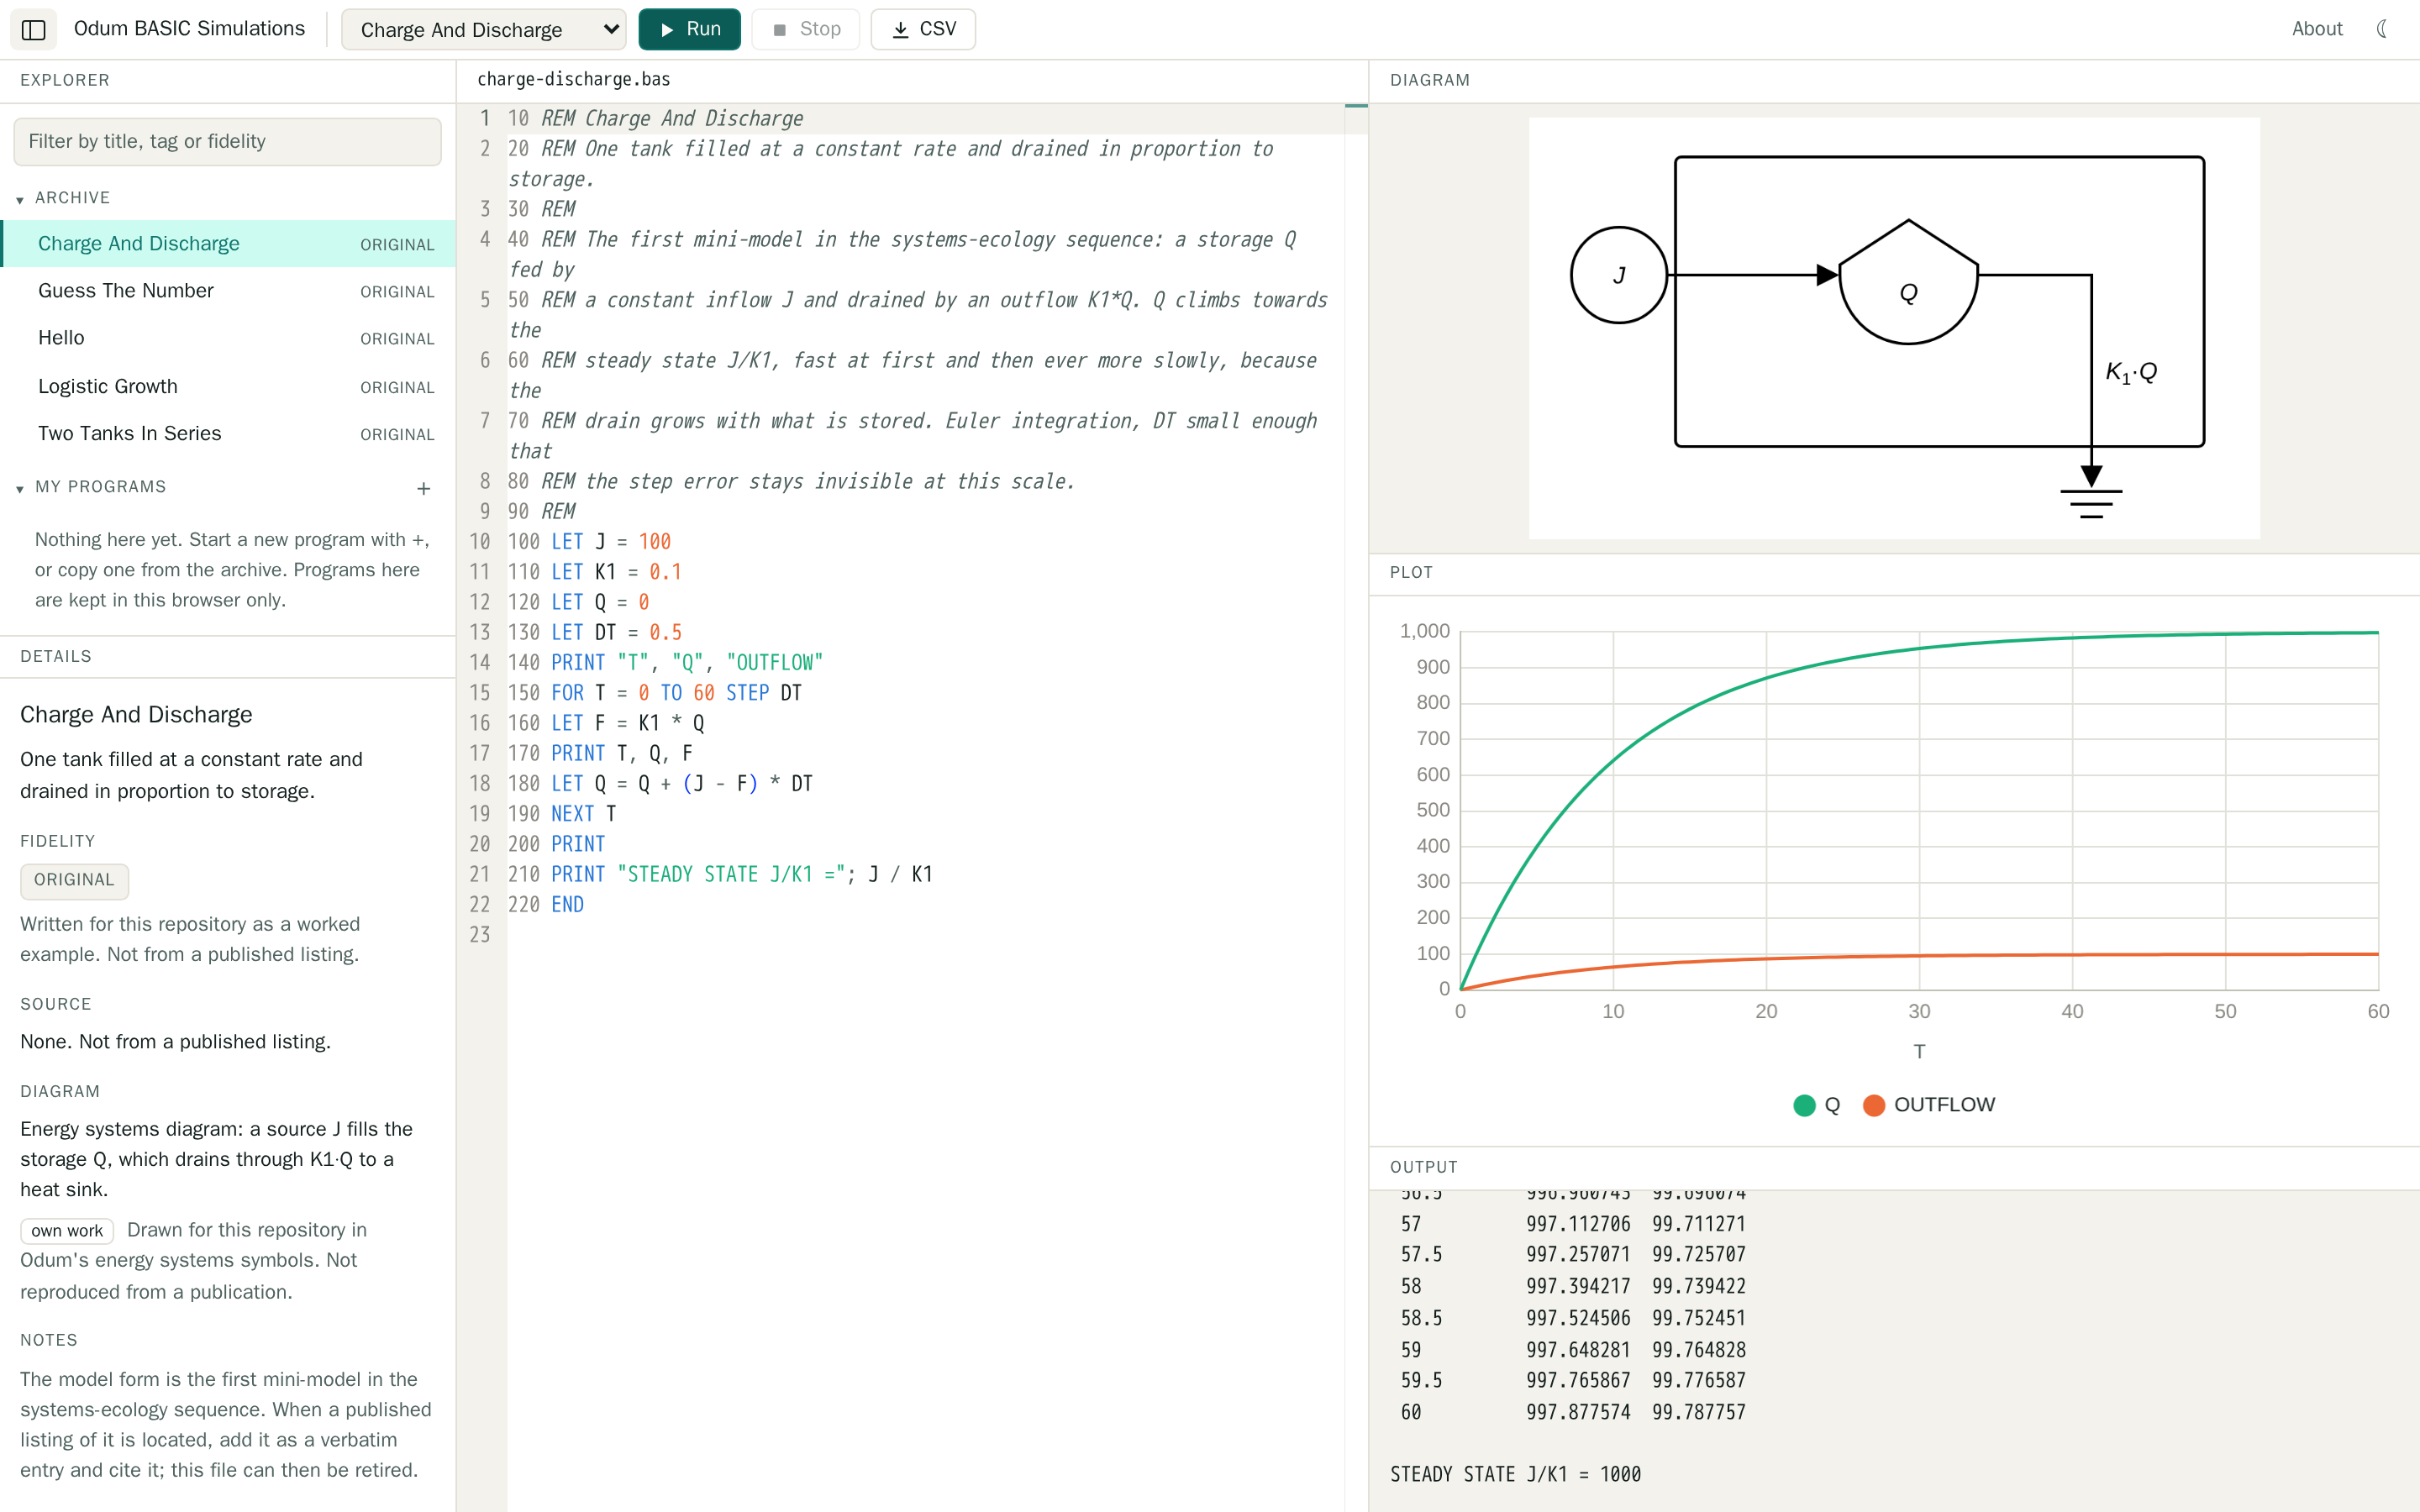
\includegraphics[width=0.88\linewidth]{workbench.png}
\caption{The browser-based workbench interface displaying the charge-and-discharge benchmark model following simulation execution, illustrating model navigation, source code editing, Energy Systems Language diagram rendering, tabular console output, and reconstructed phase trajectory plotting. The indicator at the upper right reports the state of the WebAssembly build of the C engine, which checks the listing in the editor as it is typed; it is a status of the checker alone, and simulation execution proceeds independently of it.}
\label{fig:workbench}
\end{figure}

% REVIEW(implementation/website): nothing in this section says how any of this
% reaches the site, which is a gap given the paper is about a browser runtime.
% What happens now, and is worth a short paragraph here:
%
%   - engine.wasm is fetched once per page and instantiated in the browser.
%     BAS_Validate returns diagnostics already in the editor's marker shape, so
%     they are passed through untranslated rather than converted.
%   - The editor checks the listing as it is typed (debounced), so a reader
%     editing a historical listing is told where it stops being valid BASIC.
%   - The same engine backs the command-line tool's `check`, so the editor and
%     the tool agree by construction rather than by two implementations being
%     kept in step. That is an architectural claim the paper should make.
%   - It fails open: if the module cannot be fetched the editor keeps working
%     without marks, because an editor that refuses to open because a checker is
%     missing is worse than an unchecked one. The topbar indicator in Figure 1
%     reports which state it is in.
%   - The build emits no JavaScript glue (-sSTANDALONE_WASM, --no-entry); the
%     only import is a memory-growth notice, because the validation path touches
%     no stdio and so pulls in no WASI. Worth one clause: it is what keeps the
%     committed artefact reviewable.
Automated extraction of quantitative trajectories from legacy console output requires a systematic heuristic. Because historical simulation listings predate structured data-interchange formats, simulation results were sequentially emitted via formatted \texttt{PRINT} statements. The extraction engine scans the output stream for contiguous blocks of multi-column numeric data delimited by standard whitespace or tab tokens. The longest contiguous block sharing a constant field width is classified as the primary simulation table, with the initial column designated as the independent temporal variable. Column headers are automatically parsed from preceding non-numeric string labels. If the parsing heuristic fails to detect a consistent tabular structure, raw text streams remain fully accessible to the user, and resolved tables may be exported as standardized comma-separated values (CSV).

\begin{figure}[t]
\centering
\begin{subfigure}[b]{0.48\linewidth}
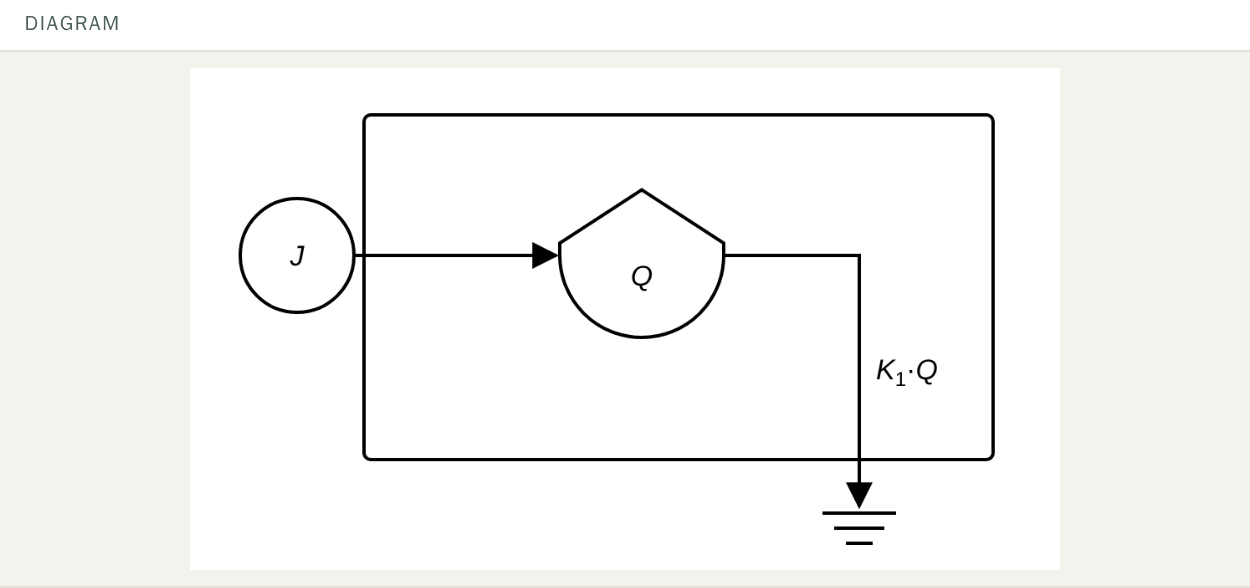
\includegraphics[width=\linewidth]{minimodel-diagram.png}
\caption{Energy Systems Language diagram.}
\end{subfigure}\hfill
\begin{subfigure}[b]{0.48\linewidth}
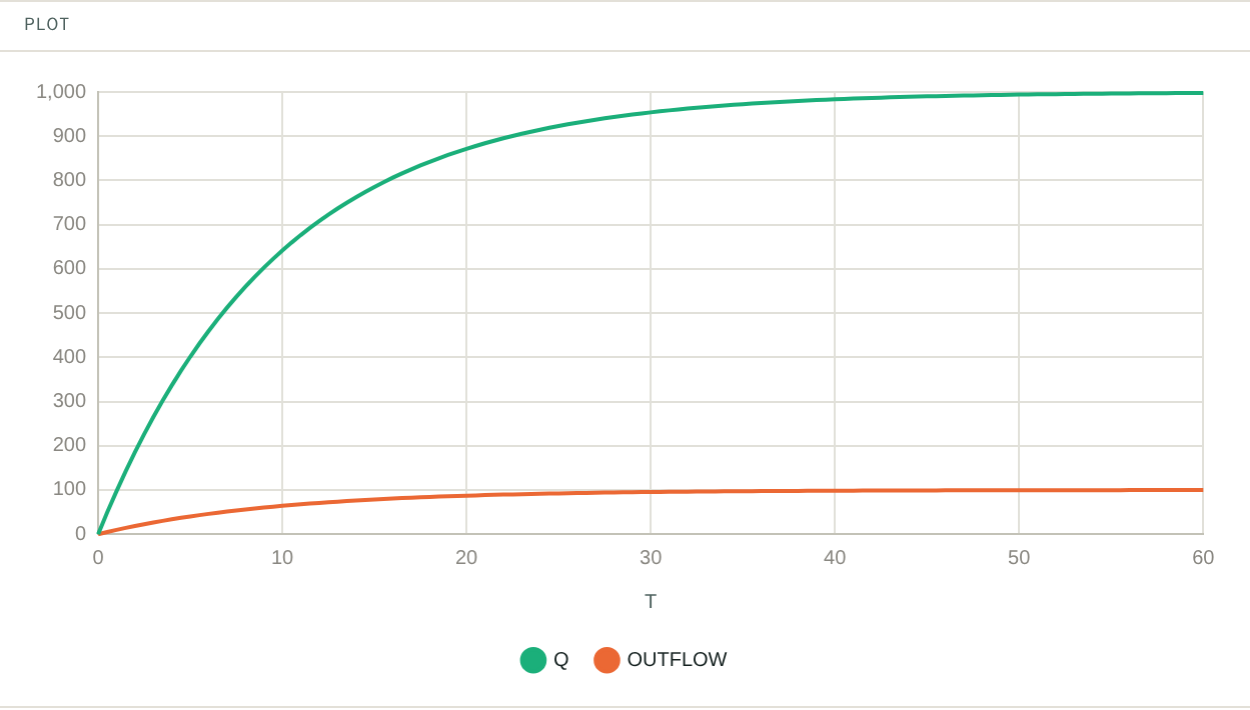
\includegraphics[width=\linewidth]{minimodel-plot.png}
\caption{Reconstructed simulation trajectory.}
\end{subfigure}
\caption{Dual representation of an ecological compartmental model within the archive: (a) visual Energy Systems Language diagram indicating forcing function $J$, storage $Q$, and donor-controlled outflow $K_1Q$; (b) corresponding dynamic trajectory recovered directly from the interpreted forward-Euler numerical integration output.}
\label{fig:minimodel}
\end{figure}

The graphical workbench interface integrates these execution facilities into a unified analytical environment (Figure~\ref{fig:workbench}). The interface organizes models within an interactive catalog, displaying source listings alongside corresponding Energy Systems Language diagrams, recovered dynamic plots, and console execution logs (Figure~\ref{fig:minimodel}). Each program is addressable via persistent uniform resource identifiers, ensuring stable cross-referencing for scientific and educational applications.

The archival filesystem hierarchy enforces strict isolation between program definitions and relational metadata. Program modules are cataloged within a structured directory hierarchy containing legacy listings (\texttt{.bas}), standardized metadata specification files (\texttt{.json}), and accompanying raster diagrams. Published volumes containing multiple minimodels are aggregated into cohesive directory modules linked to master bibliographic records. Automated build pipelines enforce schema compliance across all entries, verifying that directory structures match declared citation keys and that modification diffs are preserved without altering verbatim source texts.

%% ----------------------------------------------------------------------------
\section{Ingestion workflows and provenance verification}
\label{sec:contributing}

To facilitate the expansion of the historical model corpus while maintaining archival integrity, the framework provides four ingestion pathways calibrated to varying technical requirements (Figure~\ref{fig:routes}, Table~\ref{tab:routes}).

\begin{table}[h]
\centering\small
\begin{tabularx}{\linewidth}{@{}lXXX@{}}
\toprule
Ingestion pathway & User technical prerequisites & Automated validation & Human verification protocol \\
\midrule
Version-control pull request & Git version-control; JSON schema compliance & Static build validation; regression test harness & Code review; bibliographic verification \\
Structured issue form & Standard web access; repository account & Automated schema compilation and linting & Review of attached source documentation; approval \\
Interactive workbench & Client web browser & Dynamic schema validation; pre-filled issue staging & Visual comparison against primary literature scan \\
Automated transcription & Source scan or transcription prompt & Automated parsing; syntax check; test execution & Mandatory verification of numerical coefficients against original page \\
\bottomrule
\end{tabularx}
\caption{Summary of archival ingestion pathways, detailing operational prerequisites, automated validation routines, and human verification checkpoints.}
\label{tab:routes}
\end{table}

The primary pathway utilizes formal version-control pull requests, enabling advanced contributors to supply complete program packages comprising source listings, diagram assets, and metadata files. Continuous integration pipelines validate all companion metadata files against the central JSON schema and run regression test suites prior to human code review.

\begin{figure}[t]
\centering
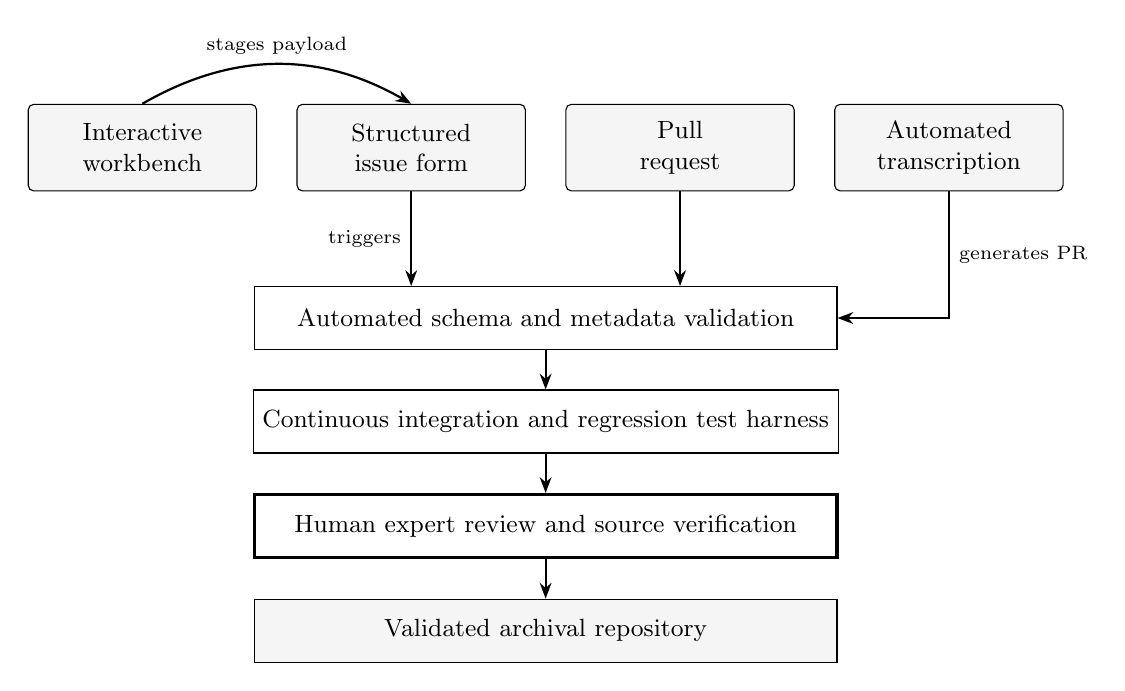
\begin{tikzpicture}[
  node distance=5mm and 5mm,
  every node/.style={font=\small, align=center},
  entry/.style={draw, rounded corners=2pt, minimum width=29mm, minimum height=11mm, fill=gray!8},
  stage/.style={draw, minimum width=74mm, minimum height=8mm},
  human/.style={stage, very thick},
  flow/.style={-{Stealth[length=2mm]}, thick},
]
\node[entry] (ws) {Interactive\\workbench};
\node[entry, right=of ws] (form) {Structured\\issue form};
\node[entry, right=of form] (pr) {Pull\\request};
\node[entry, right=of pr] (jules) {Automated\\transcription};
\node[stage, below=12mm of $(form.south)!0.5!(pr.south)$] (val) {Automated schema and metadata validation};
\node[stage, below=of val] (ci) {Continuous integration and regression test harness};
\node[human, below=of ci] (rev) {Human expert review and source verification};
\node[stage, below=of rev, fill=gray!8] (arc) {Validated archival repository};
\draw[flow] (ws.north) to[bend left=30] node[above, font=\scriptsize] {stages payload} (form.north);
\draw[flow] (form.south) -- node[left, font=\scriptsize] {triggers} (val.north -| form.south);
\draw[flow] (pr.south) -- (val.north -| pr.south);
\draw[flow] (jules.south) |- node[pos=0.25, right, font=\scriptsize] {generates PR} (val.east);
\draw[flow] (val) -- (ci);
\draw[flow] (ci) -- (rev);
\draw[flow] (rev) -- (arc);
\end{tikzpicture}
\caption{Architectural schema of the ingestion and verification pipeline, illustrating automated validation, continuous integration testing, and human-in-the-loop review criteria across all four contribution pathways.}
\label{fig:routes}
\end{figure}

To lower technical barriers for domain specialists in ecology who may not utilize distributed version-control tools, a secondary pathway leverages structured issue forms. Contributors submit program listings, bibliographic data, and visual scans through standardized web form fields. An automated repository workflow parses the submitted issue payload, compiles the corresponding metadata files, and triggers the central validation suite. Diagnostic feedback is returned automatically if required parameters are missing or malformed. Once validation succeeds, an automated pull request is generated, preserving contributor attribution while staging the submission for human verification.

The third pathway operates within the interactive workbench. Contributors draft, execute, and annotate models within a private local browser workspace. The interface performs continuous schema validation during editing. Upon completion, the workspace compiles the metadata and redirects the user to the structured submission form with all fields pre-populated, preventing manual formatting errors.

A fourth ingestion pathway accommodates automated transcription from digitized document scans. Because automated optical character recognition can introduce subtle numerical inaccuracies in mathematical coefficients without generating syntax errors, this pathway is constrained by strict oversight protocols: automated transcription agents are restricted to clerical code extraction, and repository maintainers are required to perform line-by-line manual verification against primary source scans before merging.

Diagram preservation requires distinct intellectual property governance. The archive records formal rights statements for every visual asset, cataloging the reproduction basis (e.g., author-created, public domain, authorized permission, or fair-use scholarship review) alongside precise page and figure attributions. Binary diagram formats are restricted to static raster representations (PNG, JPEG) to prevent security risks associated with executable script contexts in vector formats.

%% ----------------------------------------------------------------------------
\section{AI-assisted implementation and verification methodology}
\label{sec:llm}

In accordance with institutional guidelines governing the disclosure of artificial intelligence technologies in scientific research \citep{elsevierAI}, this section details the formal protocols, toolchains, and test-driven validation criteria employed during the development of the execution runtime.

The runtime architecture, parsing modules, and metadata validation suites were implemented utilizing Claude Code \citep{claudeCode}, an agentic development tool operating with the Claude Opus~5 language model, under continuous human direction. The methodological division of responsibility maintained human ownership over system architecture, mathematical formulations, dialect precedence rules, and intellectual property governance, while leveraging the language model for rapid code drafting, test construction, and documentation synthesis. Direct automated modifications to production branches were prohibited: all generated code was committed to isolated task branches and required successful passage through automated regression harnesses and human code review prior to integration.

To mitigate known failure modes associated with automated code generation—including hallucinated language features, silent numerical edge-case failures, and architectural regression—the development lifecycle enforced five procedural controls:
\begin{enumerate}
\item \textbf{Specification-first test-driven implementation:} Explicit unit assertions and behavioral expectations were defined prior to the synthesis of functional runtime modules.
\item \textbf{Dual-layer integration testing:} Automated test pipelines executed test suites across both raw development sources and compiled, bundled deployment packages to detect toolchain-induced discrepancies.
\item \textbf{Isolated development worktrees:} Concurrent programming tasks were executed within segregated git worktrees, preventing cross-task state contamination.
\item \textbf{Machine-checkable visual regression testing:} Automated browser automation harnesses captured rendered interface states against pinned golden reference images, verifying that visual outputs, plotting canvases, and layout structures remained invariant across modifications.
% REVIEW(llm/controls): a sixth control now exists and is the strongest of
% them: the attestation. `make attest` regenerates every result in
% validation/oracle/ from scratch inside digest-pinned containers and compares
% each against a recorded SHA-256, and a `wasm` job rebuilds the committed
% WebAssembly artefact and fails if a byte moved. Both run on every pull
% request. The distinction worth drawing is that controls 1-5 check that the
% code does what a test says, whereas this checks that published numbers can
% still be regenerated -- which is the property the paper is about.
\item \textbf{Granular commit auditing:} Machine-assisted commits incorporated standardized co-author trailers, providing an immutable audit trail of automated contributions within the repository history.
\end{enumerate}

% REVIEW(llm/efficacy): this paragraph reports only failures the controls
% caught, which overstates them. A defect reached the deployed site and is worth
% reporting honestly, because it is a failure mode specific to this methodology:
%
%   The C engine selected a statement type by arithmetic on the keyword
%   enumeration -- `map[kw - BAS_KW_DIM]`. INPUT does not sit beside DIM in that
%   enumeration, so the subtraction underflowed as an unsigned index, passed the
%   bounds check, and selected entry zero: every INPUT was parsed as a DIM. It
%   validated clean wherever the statement resembled a DIM, which `INPUT G`
%   does, so nothing failed until `INPUT "YOUR GUESS"; G` -- the form used by an
%   archived listing -- was checked, and the editor then reported a published
%   listing as broken. Two releases shipped in that state.
%
%   The test that should have caught it asserted that "every published listing
%   must pass the checker", and then checked one listing. The control was
%   present and the assertion was wrong: a sample of one, written as a
%   guarantee about a corpus. The fix was to check the whole corpus, and the
%   regression guard was confirmed to fail against the previously committed
%   artefact before it was allowed to pass.
%
% This is a more useful methodological finding than the two successes already
% reported, and it qualifies the claim in the closing sentence of this section:
% test harnesses bound what a model can silently get wrong only to the extent
% that the assertions say what the author believes they say.
The efficacy of these validation controls was evaluated empirically against subtle implementation errors encountered during runtime construction. For example, integration testing identified an unhandled temporal index offset in a synthetic two-tank benchmark listing, wherein an inflow termination condition was evaluated subsequent to state integration, shifting effective cutoff timing by two integration intervals. Similarly, during the implementation of graphics coordinate transformations, regression testing revealed discrepancies in midpoint coordinate rounding between modern floating-point conversions and legacy PC rasterization routines. In each instance, automated test failures or explicit source discrepancies halted integration, necessitating human architectural intervention. These observations reinforce established findings in empirical software engineering: while automated language models demonstrate high proficiency in generating localized algorithms to formal specifications \citep{chen2021}, their deployment in complex systems requires formal testing harnesses and human domain expertise to ensure scientific integrity \citep{jimenez2024}.

\begin{table}[h]
\centering\small
\begin{tabularx}{\linewidth}{@{}Xr@{}}
\toprule
Architectural component & Metric count \\
\midrule
Pull requests integrated & 17 \\
Non-merge development commits & 24 \\
TypeScript source lines (interpreter core and utilities) & 5{,}899 \\
\quad of which dedicated to the BASIC interpreter engine & 1{,}024 \\
Styling and interface markup lines & 1{,}920 \\
Automated test suite volume (lines of test code) & 3{,}476 \\
Unit test assertions & 218 \\
End-to-end integration test assertions (development and release builds) & 96 \\
Visual regression golden assertions & 3 \\
\bottomrule
\end{tabularx}
% REVIEW(llm/table): every count is stale, and the C engine is missing
% entirely. Measured at 56a43e8 -- regenerate before submission rather than
% copying these:
%
%   Pull requests integrated          17 -> 28
%   Non-merge development commits     24 -> 41
%   TypeScript source lines        5,899 -> 6,578
%     of which the BASIC interpreter 1,024 (unchanged)
%   Unit test assertions             218 -> 226
%   End-to-end assertions             96 -> 113 (56 tests over two projects)
%   Visual regression goldens          3 -> 4
%
% Rows the table does not have and needs, since the C engine is a headline
% contribution: C engine source and headers, 2,273 lines; C engine tests, 645
% lines (51 assertions across three suites); the committed WebAssembly artefact,
% 52 KB. Also consider a row for the attestation, which is 32 recorded results.
\caption{Quantitative structural metrics of the reconstructed execution framework and validation test harness, derived from the version-controlled release repository.}
\label{tab:llm}
\end{table}

% REVIEW(llm/ratio): "over 37%" is computed from the stale figures above and
% excludes the C engine's tests entirely. Recompute from the corrected table.
The resulting codebase (Table~\ref{tab:llm}) maintains a substantial ratio of verification logic to runtime logic, with automated test harnesses comprising over 37\% of the total codebase volume. This extensive testing infrastructure provides the empirical basis for trusting a computational engine constructed through AI-assisted development methodologies.

%% ----------------------------------------------------------------------------
\section{Validation and numerical analysis}
\label{sec:validation}

% REVIEW(validation/tiers): "three complementary lines" no longer enumerates
% what the section contains. Independent reimplementation (R5) is now argued in
% sec 7.2, but it is a different kind of evidence from emulator agreement: an
% emulator constrains shared error only insofar as it shares no ancestry with
% the interpreter, whereas a second implementation written from the same
% specification tests that directly. Either promote it to a fourth tier with its
% own subsection and say so here, or state explicitly that tier two now has two
% components. Leaving the count at three while the text carries four arguments
% is the one option to avoid.
Evaluating the reliability of the reconstructed runtime requires three complementary lines of empirical evidence: comparative verification against analytical solutions of canonical ecological systems, cross-platform validation against emulated historical interpreters, and concordance testing against historical printed outputs.

\subsection{Analytical verification on canonical compartmental models}

The initial validation tier evaluates the numerical execution engine against three canonical compartmental models characterized by closed-form analytical solutions:
\begin{enumerate}
\item \textbf{Linear charge-and-discharge storage:} A single-state reservoir governed by constant input flux $J$ and linear, donor-controlled drainage $K_1Q$:
\begin{equation}
\frac{\mathrm{d}Q}{\mathrm{d}t} = J - K_1Q, \quad Q(t) = \frac{J}{K_1}\left(1 - e^{-K_1t}\right).
\end{equation}
\item \textbf{Logistic growth resource model:} A self-limiting biological population exhibiting density-dependent saturation:
\begin{equation}
\frac{\mathrm{d}Q}{\mathrm{d}t} = K_1Q(S_T - Q) - K_2Q, \quad Q(t) = \frac{C}{1 + \left(\frac{C - Q_0}{Q_0}\right)e^{-rt}},
\end{equation}
where intrinsic growth rate $r = K_1S_T - K_2$ and carrying capacity $C = S_T - K_2/K_1$.
\item \textbf{Two-stage linear cascade with step forcing:} A coupled linear system ($\mathrm{d}Q_1/\mathrm{d}t = J - K_1Q_1$, $\mathrm{d}Q_2/\mathrm{d}t = K_1Q_1 - K_2Q_2$) subject to a piecewise step-down in forcing $J$ at time $t_c$, yielding exponential decay phases across both state variables.
\end{enumerate}

Each model listing executes an explicit forward-Euler integration recurrence over discrete time increments $\Delta t$. In automated validation tests, the interpreter output was compared across every time step against an independent recurrence evaluation executed in identical operational sequence, as well as against the analytical solution (Table~\ref{tab:validation}).

\begin{table}[h]
\centering\small
\begin{tabular}{@{}lrrcc@{}}
\toprule
& & & \multicolumn{2}{c@{}}{Maximum relative error} \\
\cmidrule(l){4-5}
Benchmark model & $\Delta t$ & Output rows & Interpreter vs.\ recurrence & Recurrence vs.\ analytical \\
\midrule
Linear charge-and-discharge & 0.50 & 121 & $\le 5\times10^{-7}$ & 0.94\% \\
Logistic growth & 0.50 & 401 & $\le 5\times10^{-7}$ & 7.41\% \\
Coupled linear cascade ($t_c = 40.5$) & 0.25 & 321 & $\le 5\times10^{-7}$ & 0.70\% \\
Coupled linear cascade ($t_c = 40.0$, nominal) & 0.25 & 321 & $\le 5\times10^{-7}$ & 7.27\% \\
\bottomrule
\end{tabular}
\caption{Numerical validation of the reconstructed interpreter across canonical compartmental models. Discrepancies between interpreter output and independent forward-Euler recurrences fall strictly within the six-digit formatting rounding threshold ($5\times10^{-7}$). Discrepancies between recurrence sequences and exact analytical solutions reflect standard discretization truncation errors inherent to first-order Euler integration.}
\label{tab:validation}
\end{table}

% REVIEW(validation/precision): this tier's tolerance depends on an assumption
% the paper does not state -- that the interpreter and the reference recurrence
% use the same arithmetic. Both are double precision today, so the $5\times
% 10^{-7}$ threshold is the display rounding alone. If execution moves to the C
% engine, that stops being true, and the number is worth recording now because
% it decides whether such a move is viable:
%
%   C engine vs. a single-precision reference recurrence   4.9e-7  (inside)
%   C engine vs. the present double-precision reference    1.16e-4 (232x over)
%
% The gap is about one float32 unit in the last place of the peak value
% (1.16e-7 of peak, against 2^-23 = 1.19e-7), so it is precision itself and not
% instability. The consequence is that moving execution to single precision does
% NOT require loosening this tolerance; it requires computing the reference
% recurrence in single precision too, which is what the original machine did.
% The claim then strengthens -- fidelity to the machine rather than to a
% double-precision idealisation -- and the threshold stays where it is.
Across all evaluated rows, the interpreter output coincided with the independent numerical recurrence to within the six-digit rounding threshold of the console display routine ($\le 5\times10^{-7}$). The remaining deviations between the numerical trajectories and the analytical benchmarks represent standard numerical truncation error characteristic of first-order forward-Euler integration: below 1\% for the linear models, and 7.41\% for the logistic model, whose effective parameter product ($r\Delta t = 0.19$) introduces greater discretization error. In the coupled cascade model, evaluating the nominal listing exposed an execution timing offset: because the conditional termination statement (\texttt{IF T > 40 THEN LET J = 0}) was sequenced following state updates, the effective inflow cut occurred at $t = 40.5$ rather than $t = 40.0$, elevating analytical error from 0.70\% to 7.27\%. Preserving such anomalies within the archive illustrates the necessity of executing listings directly rather than relying on textual descriptions.

\subsection{Cross-platform validation against emulated historical runtimes}

The second validation tier examines the numerical and graphical correspondence between the reconstructed runtime and an emulated historical execution environment. The evaluation examined a published systems ecology listing modeling macroeconomic-resource interactions over 640 forward-Euler integration steps with state-dependent threshold switching \citep[Table~3]{odum1989}. The model was executed simultaneously within the reconstructed web runtime and within PC-BASIC \citep{pcbasic}, an open-source emulator that replicates GW-BASIC architecture and Microsoft Binary Format floating-point representations.

\begin{table}[h]
\centering\small
\resizebox{\linewidth}{!}{\oracleTable}
\caption{Comparative numerical evaluation of Odum (1989, Table~3) across 640 forward-Euler integration steps executed within the reconstructed interpreter (R1, R4a, R4b) and the PC-BASIC reference emulator (R2, R3, R3d). The maximum relative difference reflects deviations across all state variables. Plotted pixel agreement indicates coordinate identity across all 2,560 trajectory points. Bit-identical steps quantify exact binary floating-point concordance with the single-precision emulator reference.}
\label{tab:oracle}
\end{table}

Because the reconstructed interpreter computes using IEEE-754 double-precision arithmetic whereas GW-BASIC utilized MBF single-precision by default, divergence between modern and historical trajectories could arise from numerical precision differences. However, as documented in Table~\ref{tab:oracle}, precision divergence does not alter macro-scale model behavior. The maximum relative difference between modern double-precision execution and legacy single-precision emulation remained bounded at $4.0\times10^{-5}$, primarily localized in a state variable constrained to a minimum floor of 0.0001. Across all 2,560 plotted trajectory coordinates, screen-space displacement did not exceed $6.8\times10^{-5}$ pixels, resulting in 100\% visual pixel concordance across the rendered trajectories. Furthermore, dynamic threshold switching (\texttt{IF D > 30 THEN IV = 0}) occurred identically at step 263 ($t = 131.5$) across all execution environments. When double-precision variables were emulated within the reference platform (Run R3d), numerical concordance reached $3.7\times10^{-13}$, verifying that the statement semantics of the interpreter introduce no algorithmic distortion.

\begin{figure}[h]
\centering
\begin{subfigure}{0.48\linewidth}

\includegraphics[width=\linewidth]{r2.png}
\caption{Reference emulator screen output}
\end{subfigure}\hfill
\begin{subfigure}{0.48\linewidth}

\includegraphics[width=\linewidth]{r1-diff.png}
\caption{Reconstructed display difference map}
\end{subfigure}
\caption{Comparative rasterization analysis of Odum (1989, Table~3) in \texttt{SCREEN 1} mode (320$\times$200 pixels). (a) Emulated video buffer output generated by PC-BASIC. (b) Reconstructed canvas output, with 111 differing pixels highlighted in white. The discrepancy was traced to divergent midpoint rounding conventions between the emulator and primary GW-BASIC interpreter source code.}
\label{fig:oracle}
\end{figure}

Cross-platform raster comparison revealed an informative implementation divergence. Comparing the emulated video memory of PC-BASIC with the reconstructed canvas buffer identified an apparent spatial mismatch across 111 of 64,000 pixels (Figure~\ref{fig:oracle}). Emulating single-precision arithmetic did not alter this mismatch, indicating that the variation arose from coordinate discretization rather than numerical drift. Analysis revealed that the temporal increment of 0.5 units mapped alternate integration steps exactly to half-pixel coordinates. PC-BASIC's rasterization routine rounded half-integers to the nearest even integer (round-half-to-even), whereas the reconstructed runtime rounded half-integers away from zero. 

Applying the hierarchical evidentiary criteria defined in Section~\ref{sec:design}, this conflict was arbitrated through examination of primary source artifacts. Within the released assembly source code of GW-BASIC \citep{gwbasic}, graphics coordinate conversion calls the internal routine shared by the integer conversion function \texttt{CINT}, which implements symmetric round-half-away-from-zero rounding. Consequently, the reconstructed runtime's coordinate mapping conformed to the historical hardware implementation, whereas the emulator exhibited an undocumented internal deviation. Resolving this discrepancy demonstrates the value of multi-engine comparative validation in computational software archaeology.

A reconstructed runtime that recovers a historical trajectory establishes that the trajectory is recoverable; it does not establish that the recovery is independent of the particular program performing it. A systematic error in the interpreter would be reproduced faithfully by every run of that interpreter, and agreement with an emulator constrains this only insofar as the two share no common ancestry. To separate these, the language core was implemented a second time, in C, and compiled both to a native command-line executable and to WebAssembly for in-browser use. The second implementation computes in single precision by type rather than in double precision, and enforces its arithmetic contract at compile time: intermediate results may not be evaluated at wider precision (\texttt{FLT\_EVAL\_METHOD} equal to zero), and floating-point contraction is disabled, so that a fused multiply-add cannot round once where the original rounded twice.

Executing the same listing through this implementation (Run R5) and rasterizing its output through the display routine shared with the primary interpreter yields a screen differing from that interpreter's in \oracleEnginesDiffering{} of \oracleScreenPixels{} pixels, and differing from the PC-BASIC reference in \oracleEngineScreenDiffering{}---the identical disparity exhibited by the primary interpreter, and attributable to the same midpoint rounding convention analyzed above. Rounding to single precision after every operation within the TypeScript interpreter likewise alters \oraclePrecisionsDiffering{} pixels. Two independently written implementations, in different languages and at different arithmetic precisions, therefore reconstruct the published figure identically, which localizes the residual disparity in the rasterization convention rather than in either interpreter or in the choice of numeric format. This comparison is regenerated and verified on every proposed change to the repository, so the agreement is a maintained property rather than a single historical measurement.

The third tier of validation—direct automated verification against original printed output tables and published figure scans—represents an ongoing empirical objective that requires progressive expansion of the verified listing corpus.

%% ----------------------------------------------------------------------------
\section{Discussion}
\label{sec:discussion}

The restoration of execution fidelity to historical ecological models provides a rigorous computational foundation for evaluating early systems ecology literature. In computational science, publishing source code listings without an active runtime provides incomplete reproducibility; when software environments decay, scientific claims become unfalsifiable. By reconstructing an open, web-accessible execution environment, historical simulation listings are transformed from static typographical records into active computational experiments that can be verified, audited, and extended.

This capability facilitates several investigative avenues in systems ecology:
\begin{itemize}
\item \textbf{Direct verification of published trajectories:} Researchers can independently evaluate whether published forward-Euler algorithms faithfully reproduce the phase behaviors and transient responses depicted in printed figures. Discrepancies between printed narratives and algorithmic behavior—such as the step-forcing timing offset observed in Section~\ref{sec:validation}—can be identified and documented rather than obscured by modern re-implementations.
\item \textbf{Pedagogical accessibility:} Students and researchers can interact directly with historical models within a standardized browser environment, exploring parameter sensitivities and dynamic properties without requiring specialized emulation toolchains or obsolete hardware.
\item \textbf{Dual-formalism consistency testing:} In Odum's systems ecology, models were simultaneously specified as visual Energy Systems Language diagrams and as executable differential equations. Because visual and mathematical formalisms can drift apart during publication, a verified execution archive provides an essential empirical benchmark for evaluating automated diagram-to-model compilation environments \citep{energese,gssk}.
\end{itemize}

From a software preservation perspective, this investigation highlights a fundamental methodological distinction between software evolution analysis and runtime reconstruction. Standard software archaeology interrogates dynamic repositories to trace code modifications over time \citep{huntThomas2002,robles2005,spinellis2021}. For historical scientific listings, the preservation target is not an evolving code repository but an immutable printed artifact whose operational context has dissolved. Preserving such models requires an evidential approach to runtime reconstruction, governed by strict source hierarchies and transparent provenance tracking.

The introduction of formal fidelity classifications (Table~\ref{tab:fidelity}) addresses an important omission in contemporary research software preservation frameworks. While the FAIR4RS guidelines \citep{barker2022} define essential criteria for discoverability and licensing, they presume that preserved code represents an authentic primary artifact. In historical computational recovery, distinguishing between verbatim transcriptions, errata-corrected listings, and modern algorithmic adaptations is paramount. Standardizing fidelity metadata ensures that scientific users can clearly differentiate between historical modeling artifacts and contemporary enhancements.

Similarly, establishing explicit rights metadata for accompanying visual diagrams provides a structured framework for managing intellectual property in scientific archives. While computational algorithms expressing scientific equations occupy distinct legal copyright parameters, visual diagrams require explicit attribution and rights declarations. Incorporating per-figure rights metadata balances open scientific dissemination with rigorous copyright compliance.

\subsection{Limitations and future research}

Several technical boundaries bound the current implementation:
\begin{enumerate}
\item \textbf{Language dialect coverage:} The current interpreter core supports the standard procedural and graphical statements characteristic of Odum's minimodels, but omits advanced structured control constructs (\texttt{WHILE/WEND}, \texttt{SELECT CASE}) and specialized string-formatting commands (\texttt{PRINT USING}, \texttt{LOCATE}). Expanding dialect coverage is required to accommodate larger simulation listings.
% REVIEW(limitations): the dialect-coverage item above lists what the
% TypeScript interpreter omits, but the C engine's gaps are larger and more
% consequential, because they are what currently prevents a single
% implementation from serving the whole system. Add them:
%   - INPUT is not implemented, and implementing it is not just a missing case:
%     it must suspend and resume across BAS_Step, and BAS_Status has no value
%     meaning "waiting for input", so it is an API change.
%   - PRINT emits numeric rows and drops string literals by design, so the
%     engine produces no console text and the table heuristic has nothing to
%     read.
% Until both exist, the site runs programs on the TypeScript interpreter and
% checks them with the C engine. A reader should be told that, and told that
% moving execution across would also move the arithmetic to single precision --
% see the note at the validation section.
\item \textbf{Empirical corpus expansion:} The present study validates the runtime architecture primarily against canonical benchmark models and selected historical listings. Transcribing, validating, and cataloging the extensive corpus of models distributed across Odum's foundational texts \citep{odum1983,odumMinimodels,odumOdum2000} constitutes an ongoing archival effort.
\item \textbf{Automated raster validation:} While graphical outputs can be rendered and compared at the pixel level, automated validation against historical scanned diagrams requires the development of robust visual comparison metrics that account for paper aging, print distortions, and scanner artifacts.
\end{enumerate}

%% ----------------------------------------------------------------------------
\section{Conclusions}
\label{sec:conclusions}

The computational preservation of historical scientific literature requires restoring the execution environments upon which computational claims depend. H.T. Odum and his collaborators documented systems ecology through fully disclosed, executable BASIC programs, yet the obsolescence of vintage computing environments rendered these models historically inaccessible.

% REVIEW(conclusions): the summary stops at emulator agreement and omits the
% independent-reimplementation result, which is the conclusion best supported by
% the evidence: two implementations, two languages, two arithmetic precisions,
% one identical screen. If the abstract is revised, revise this in step.
Odum BASIC Simulations addresses this challenge by providing an open-source, web-standard execution runtime and archival repository that executes historical simulation listings without textual modernization. By enforcing machine-checked provenance schemas, formal fidelity taxonomies, and hierarchical evidence arbitration, the framework restores computational repeatability to historical systems ecology models. Numerical evaluations demonstrate that the reconstructed runtime achieves exact arithmetic concordance with legacy forward-Euler recurrences and resolves subtle historical rasterization semantics through primary interpreter source analysis. This computational framework bridges the gap between historical scientific literature and modern reproducibility standards, ensuring that foundational ecological models remain accessible for inspection, validation, and scientific inquiry.

%% ----------------------------------------------------------------------------
\section*{Software and data availability}

\begin{description}
\item[Software Title] Odum BASIC Simulations
\item[Developer] S. Maud
\item[Source Code Repository] \url{https://github.com/energese-project/Odum-basic-simulations}
\item[Operational Web Application] \url{https://energese-project.github.io/Odum-basic-simulations/}
\item[Software License] MIT License
\item[Archival Identifier] Zenodo DOI: [DOI to mint]
% REVIEW(availability): three corrections. (1) Node "version 20 or higher" is
% stale -- .node-version pins 26, and the unit suite runs TypeScript directly
% under node --test, which needs a current release. (2) Building the WebAssembly
% module needs emscripten, supplied through a digest-pinned container
% (engine/Containerfile.wasm); it is not required to run or build the site,
% because the artefact is committed, and that distinction is worth stating.
% (3) The oracle comparison needs a container runtime for PC-BASIC. None of
% these are needed by a reader who only wants to use the site.
\item[Execution Requirements] Platform-independent web runtime supporting ECMAScript 2022 standards. Development and build toolchains require Node.js (version 20 or higher) or standard OCI-compliant container environments.
% REVIEW(availability/data): mentions `make attest` but not the two things a
% reader would need in order to repeat the newer claims: `make wasm` rebuilds
% the committed WebAssembly module in the pinned toolchain, and
% `engine/build-wasm.sh --check` verifies that the committed bytes still follow
% from the source. Both run in CI on every pull request.
\item[Data and Test Corpora] All simulation models, metadata sidecar specifications, visual regression baselines, and cross-runtime verification scripts are maintained within the open-access project repository. Reference comparison datasets generated via \texttt{make attest} are archived within the \texttt{validation/oracle/} directory.
\end{description}

\section*{CRediT authorship contribution statement}
\textbf{S. Maud:} Conceptualization, Methodology, Software, Formal analysis, Validation, Investigation, Data curation, Writing -- original draft, Writing -- review \& editing.

\section*{Declaration of competing interest}
The author declares that there are no known competing financial interests or personal relationships that could have appeared to influence the work reported in this paper.

\section*{Declaration of generative AI and AI-assisted technologies in the manuscript preparation process}
During the preparation of this manuscript, the author utilized Claude Code (Anthropic; model Claude Opus~5) to assist in drafting initial section outlines, generating descriptive summaries of software metrics, and executing automated regression tests for tabular data. Following automated drafting assistance, the author critically reviewed, revised, and validated all prose, equations, and factual claims. The author takes full scholarly responsibility for the integrity and accuracy of the published work.

\section*{Acknowledgements}
The author acknowledges the foundational contributions of Howard T. Odum and Elisabeth C. Odum, whose commitment to open, fully disclosed computational modeling established the scientific heritage preserved by this project.

%% ----------------------------------------------------------------------------
\begin{thebibliography}{99}

\bibitem[Barker et~al.(2022)]{barker2022}
Barker, M., Chue Hong, N.P., Katz, D.S., Lamprecht, A.-L., Martinez-Ortiz, C., Psomopoulos, F., Harrow, J., Castro, L.J., Gruenpeter, M., Martinez, P.A., Honeyman, T., 2022. Introducing the FAIR Principles for research software. \emph{Scientific Data} 9, 622. \url{https://doi.org/10.1038/s41597-022-01710-x}

\bibitem[Brown and Ulgiati(2004)]{brown2004}
Brown, M.T., Ulgiati, S., 2004. Energy quality, emergy, and transformity: H.T. Odum's contributions to quantifying and understanding systems. \emph{Ecological Modelling} 178(1--2), 201--213. \url{https://doi.org/10.1016/j.ecolmodel.2004.03.002}

\bibitem[Chen et~al.(2021)]{chen2021}
Chen, M., Tworek, J., Jun, H., Yuan, Q., Pinto, H.P. de O., Kaplan, J., Edwards, H., Burda, Y., Joseph, N., Brockman, G., et al., 2021. Evaluating large language models trained on code. arXiv preprint arXiv:2107.03374. \url{https://doi.org/10.48550/arXiv.2107.03374}

\bibitem[ECMA(1978)]{ecma55}
ECMA, 1978. Standard ECMA-55: Minimal BASIC, 1st edition. European Computer Manufacturers Association, Geneva.

\bibitem[Eick et~al.(2001)]{eick2001}
Eick, S.G., Graves, T.L., Karr, A.F., Marron, J.S., Mockus, A., 2001. Does code decay? Assessing the evidence from change management data. \emph{IEEE Transactions on Software Engineering} 27(1), 1--12. \url{https://doi.org/10.1109/32.895984}

\bibitem[Elsevier(2026)]{elsevierAI}
Elsevier, 2026. Generative AI policies for journals. \url{https://www.elsevier.com/about/policies-and-standards/generative-ai-policies-for-journals} (accessed 18 September 2026).

\bibitem[Fortmann-Roe(2014)]{fortmannRoe2014}
Fortmann-Roe, S., 2014. Insight Maker: a general-purpose tool for web-based modeling \& simulation. \emph{Simulation Modelling Practice and Theory} 47, 28--45. \url{https://doi.org/10.1016/j.simpat.2014.03.013}

\bibitem[Grimm et~al.(2010)]{grimm2010}
Grimm, V., Berger, U., DeAngelis, D.L., Polhill, J.G., Giske, J., Railsback, S.F., 2010. The ODD protocol: a review and first update. \emph{Ecological Modelling} 221(23), 2760--2768. \url{https://doi.org/10.1016/j.ecolmodel.2010.08.019}

\bibitem[Hagemans(2026)]{pcbasic}
Hagemans, R., 2026. PC-BASIC: a free, cross-platform emulator for the GW-BASIC family of interpreters. Software, version 2.0.8. \url{https://github.com/robhagemans/pcbasic}

\bibitem[Hinsen(2019)]{hinsen2019}
Hinsen, K., 2019. Dealing with software collapse. \emph{Computing in Science \& Engineering} 21(3), 104--108. \url{https://doi.org/10.1109/MCSE.2019.2900945}

\bibitem[Hunt and Thomas(2002)]{huntThomas2002}
Hunt, A., Thomas, D., 2002. Software archaeology. \emph{IEEE Software} 19(2), 20--22. \url{https://doi.org/10.1109/52.991327}

\bibitem[Ince et~al.(2012)]{ince2012}
Ince, D.C., Hatton, L., Graham-Cumming, J., 2012. The case for open computer programs. \emph{Nature} 482, 485--488. \url{https://doi.org/10.1038/nature10836}

\bibitem[Jimenez et~al.(2024)]{jimenez2024}
Jimenez, C.E., Yang, J., Wettig, A., Yao, S., Pei, K., Press, O., Narasimhan, K., 2024. SWE-bench: Can language models resolve real-world GitHub issues? In: \emph{Proceedings of the Twelfth International Conference on Learning Representations (ICLR 2024)}, Vienna.

\bibitem[Kemeny and Kurtz(1964)]{kemenyKurtz1964}
Kemeny, J.G., Kurtz, T.E., 1964. \emph{BASIC: A Manual for BASIC, the Elementary Algebraic Language Designed for Use with the Dartmouth Time Sharing System}, 2nd edition. Dartmouth College Computation Center, Hanover, NH.

\bibitem[Lehman(1980)]{lehman1980}
Lehman, M.M., 1980. Programs, life cycles, and laws of software evolution. \emph{Proceedings of the IEEE} 68(9), 1060--1076. \url{https://doi.org/10.1109/PROC.1980.11805}

\bibitem[Maud(2026a)]{energese}
Maud, S., 2026a. energese: Odum's Energy Systems Language as a LuaLaTeX package. Software, version 0.1.0. \url{https://doi.org/10.5281/zenodo.22340275}

\bibitem[Maud(2026b)]{gssk}
Maud, S., 2026b. GSSK: General Systems Simulation Kernel. Software, version 5.3.0. \url{https://doi.org/10.5281/zenodo.22339312}

\bibitem[Microsoft(2020)]{gwbasic}
Microsoft, 2020. GW-BASIC: the 1983 source code, released under the MIT licence. \url{https://github.com/microsoft/GW-BASIC}

\bibitem[Odum(1960)]{odum1960}
Odum, H.T., 1960. Ecological potential and analogue circuits for the ecosystem. \emph{American Scientist} 48(1), 1--8.

\bibitem[Odum(1972)]{odum1972}
Odum, H.T., 1972. An energy circuit language for ecological and social systems: its physical basis. In: Patten, B.C. (Ed.), \emph{Systems Analysis and Simulation in Ecology}, Vol.~2. Academic Press, New York, pp. 139--211.

\bibitem[Odum(1983)]{odum1983}
Odum, H.T., 1983. \emph{Systems Ecology: An Introduction}. Wiley, New York, 644~pp.

\bibitem[Odum(1989)]{odum1989}
Odum, H.T., 1989. Simulation models of ecological economics developed with energy language methods. \emph{Simulation} 53(2), 69--75. \url{https://doi.org/10.1177/003754978905300205}

\bibitem[Odum(1994)]{odum1994}
Odum, H.T., 1994. \emph{Ecological and General Systems: An Introduction to Systems Ecology}. University Press of Colorado, Niwot.

\bibitem[Odum and Odum(1994)]{odumMinimodels}
Odum, H.T., Odum, E.C., 1994. \emph{Computer Minimodels and Simulation Exercises for Science and Social Studies}. Center for Environmental Policy, University of Florida, Gainesville.

\bibitem[Odum and Odum(2000)]{odumOdum2000}
Odum, H.T., Odum, E.C., 2000. \emph{Modeling for All Scales: An Introduction to System Simulation}. Academic Press, San Diego.

\bibitem[Ortega and Zanghetin(2007)]{ortega2007}
Ortega, E., Furlanetti de Lima Zanghetin, M., 2007. Computer minimodels and simulation exercises: web edition of Odum and Odum (1994). Laboratory of Ecological Engineering and Applied Computing (LEIA), Universidade Estadual de Campinas, Campinas.

\bibitem[Parnas(1994)]{parnas1994}
Parnas, D.L., 1994. Software aging. In: \emph{Proceedings of the 16th International Conference on Software Engineering (ICSE~'94)}, Sorrento, Italy, pp. 279--287. \url{https://doi.org/10.1109/ICSE.1994.296790}

\bibitem[Peng(2011)]{peng2011}
Peng, R.D., 2011. Reproducible research in computational science. \emph{Science} 334(6060), 1226--1227. \url{https://doi.org/10.1126/science.1213847}

\bibitem[Richmond(1985)]{richmond1985}
Richmond, B., 1985. STELLA: software for bringing system dynamics to the other 98\%. In: \emph{Proceedings of the 1985 International Conference of the System Dynamics Society}. System Dynamics Society, pp. 706--718.

\bibitem[Robles et~al.(2005)]{robles2005}
Robles, G., Gonzalez-Barahona, J.M., Herraiz, I., 2005. An empirical approach to software archaeology. In: \emph{Poster Proceedings of the 21st International Conference on Software Maintenance (ICSM 2005)}, Budapest, pp. 47--50.

\bibitem[Smith et~al.(2016)]{smith2016}
Smith, A.M., Katz, D.S., Niemeyer, K.E., FORCE11 Software Citation Working Group, 2016. Software citation principles. \emph{PeerJ Computer Science} 2, e86. \url{https://doi.org/10.7717/peerj-cs.86}

\bibitem[Spinellis et~al.(2021)]{spinellis2021}
Spinellis, D., Louridas, P., Kechagia, M., 2021. Software evolution: the lifetime of fine-grained elements. \emph{PeerJ Computer Science} 7, e372. \url{https://doi.org/10.7717/peerj-cs.372}

\bibitem[Anthropic(2026)]{claudeCode}
Anthropic, 2026. Claude Code. Software. \url{https://claude.com/claude-code} (accessed 18 September 2026).

\bibitem[Ventana Systems(2026)]{vensim}
Ventana Systems, 2026. Vensim. Software. \url{https://vensim.com/} (accessed 20 September 2026).

\bibitem[Wilkinson et~al.(2016)]{wilkinson2016}
Wilkinson, M.D., Dumontier, M., Aalbersberg, I.J., Appleton, G., Axton, M., Baak, A., et al., 2016. The FAIR Guiding Principles for scientific data management and stewardship. \emph{Scientific Data} 3, 160018. \url{https://doi.org/10.1038/sdata.2016.18}


\end{thebibliography}
% 
\end{document}